\documentclass[border=0.125cm]{standalone}
\usepackage{tikz}
\usetikzlibrary{positioning}
\usetikzlibrary{arrows}
\begin{document}

\definecolor{input_node}{RGB}{171,171,154}
\definecolor{dense_node}{RGB}{196,225,144}
\definecolor{dropout_node}{RGB}{222,222,222}
\definecolor{output_node}{RGB}{171,154,154}
% New colors
\definecolor{klight_green_100}{RGB}{220, 237, 200}
\definecolor{klight_green_200}{RGB}{197, 225, 165}
\definecolor{klight_green_300}{RGB}{174, 213, 129}
\definecolor{klight_green_400}{RGB}{156, 204, 101}
\definecolor{klight_green_500}{RGB}{139, 195, 74}
\definecolor{kred_100}{RGB}{255, 205, 210}
\definecolor{kred_400}{RGB}{239, 83, 80}
\definecolor{kyellow_400}{RGB}{255, 238, 88}
\definecolor{kgreen_300}{RGB}{129, 199, 132}
\definecolor{kgreen_500}{RGB}{76, 175, 80}
\definecolor{klime_green_500}{RGB}{100, 221, 23}
\definecolor{kblue_500}{RGB}{33, 150, 243}
\definecolor{kgrey}{RGB}{222,222,222}
\definecolor{korange}{RGB}{255, 152, 0}  % orange 500

\tikzset{%
  project part/.style={
    circle,
    draw,
    fill=klight_green_500,
    thick,
    minimum size=1cm
  },
  main line/.style={
    draw,
    line width=0.25mm,
    opacity=1,
    minimum size=1cm
  },
}

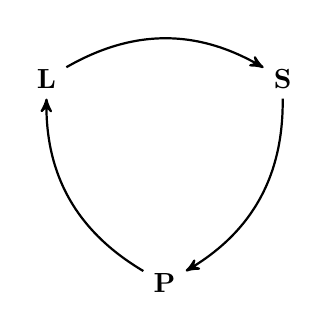
\begin{tikzpicture}[x=1.5cm, y=1.5cm, ->,>=stealth',auto, thick]
% Base project nodes
\node [project part/.try] (teacher) at (0,0) {$\textbf{L}$};
\node [project part/.try] (student) at (2,0) {$\textbf{S}$};
\node [project part/.try] (parent) at (1,-1.732) {$\textbf{P}$};

% Connect them 
\path[main line/.style={font=\sffamily\small}]
    (teacher) edge[bend left] node [right] {} (student)
    (student) edge[bend left] node [left] {} (parent)
    (parent) edge[bend left] node [above, midway] {} (teacher);
\end{tikzpicture}

\end{document}